% !TeX root = ../main.tex

% This body of work comprises much of the relevant theoretical foundations for persistent homology for data analysis in general.
We refer to the following process as \emph{topological scalar field analysis (SFA)}.
The goal is to approximate the persistent homology of a real valued function $f : D\to \R$.
The input is a sample of the function that covers its domain the domain at some scale $\delta > 0$.
A nested pair of simplicial complexes that captures the homology of the cover is then constructed on these points.
These complexes are sorted by the function values on its vertices to form a sequence of nested sub complexes known as a \emph{filtration}.
The standard reduction algorithm~\cite{edelsbrunner02simplification,zomorodian05computing} is then used to compute its persistent homology.
Stability results state that, because the vertices cover the domain at scale $\delta$, the corresponding persistence barcode is a $\delta$-approximation to that of the function itself~\cite{cohensteiner07stability,chazal09proximity}.

The primary assumption in SFA is that the sample covers the domain at some scale $\delta$.
The Peristent Nerve Theorem~\cite{chazal08towards} can then be used to show that the nested pair of simplicial captures the homology of the cover.
These nested pairs, which will be viewed as images of a map induced by inclusion, will be referred to as \emph{short filtrations}.

For a bounded $d$-dimensional domain the TCC uses the fact that the number of generators in the top-dimensional relative homology of the domain modulo its boundary is equal to the number of connected components~\cite{desilva07coverage}.
Given a finite sample $P$ and a sub-sample $Q\subseteq P$ of points near the boundary one can therefore check that the sample covers the domain at scale $\delta > 0$ by comparing number of generators in the top-dimensional relative homology of the pair $(P^\delta, Q^\delta)$ to the number of connected components of the domain.
A key observation is that this test not only confirms that the sample covers the domain, but also that we have a sub-sample of points $Q^\delta$ that resembles its boundary.
We refer to this property as being \emph{topologically representative} of the domain and its boundary.

In its original form the TCC is stated as a criteria for coverage by a sensor network in a coordinate free setting---coordinates of sensors are not provided, only some limited connectivity information.
The input is a pair of neighborhood graphs on $P$ that can be used to construct a short filtration of (Vietoris-)Rips complexes that captures the homology of the cover $(P^\delta, Q^\delta)$.
However, because there is no way to determine which points are close to the boundary analytically the TCC requires that these points $Q$ are labeled manually.
This requirement is perhaps the main reason why the TCC can so rarely be applied in practice.
It can be shown that this requirement can be removed by instead requiring that our input points sample some unknown $c$-Lipschitz function $f : D\to \R$.
This is more natural for applications to data analysis, where data represents local measurements of some underlying process.
Given a threshold $\omega\in\R$ such that the $\omega$-sub levelset $f^{-1}((-\infty,\omega])$ contains the boundary we can instead define $Q$ by function value.
The existence of this threshold, as well as additional \emph{regularity assumptions}, can then be phrased in terms of the persistent homology of the function.

% This requirement is natural for applications to data analysis, where data represents local measurements of some underlying process.
% Given a threshold on function values that can be used to define a bounding subset of the domain we can define our sampled boundary by their function values alone.
% The existence of this threshold, as well as additional \emph{regularity assumptions} that are required in order to establish the minimum resolution of the sample, can then be phrased in terms of the persistent homology of the function.
% % Moreover, the TCC requires additional \emph{regularity assumptions} that are required in order to establish the minimum resolution of the sample.
% % Traditionally, these assumptions required information about the geometry of the domain, and were made in terms of the \emph{smoothness} of its boundary.
% % Now, these assumptions can be stated directly in terms of the persistent homology of the function itself.

% Now, the TCC requires information about the persistent homology of the function.
From this perspective, information about the persistent homology of a function is required in order to confirm coverage.
Conversely, approximating the persistent homology of a function requires coverage.
In fact, the persistence computation and the TCC overlap in a number of ways.
The coverage condition can therefore be extracted directly from the approximated diagram persistence diagram, and the quality of the approximation depends on coverage.
Not only is the criterion encoded in this diagram, but its computation produces a \emph{fundamental class} for the domain that can be used to compute topological duals.
It is in this way that one can verify that a persistence diagram is representative of the scalar field by leveraging topological priors similar to those required by the TCC.
Moreover, the use of relative homology and duality in the TCC can be used to extend SFA to the setting of \emph{partial coverage}.

\begin{figure}[htbp]
% \begin{wrapfigure}{r}{0.4\textwidth}
  \centering
  % \vspace{-4ex}
  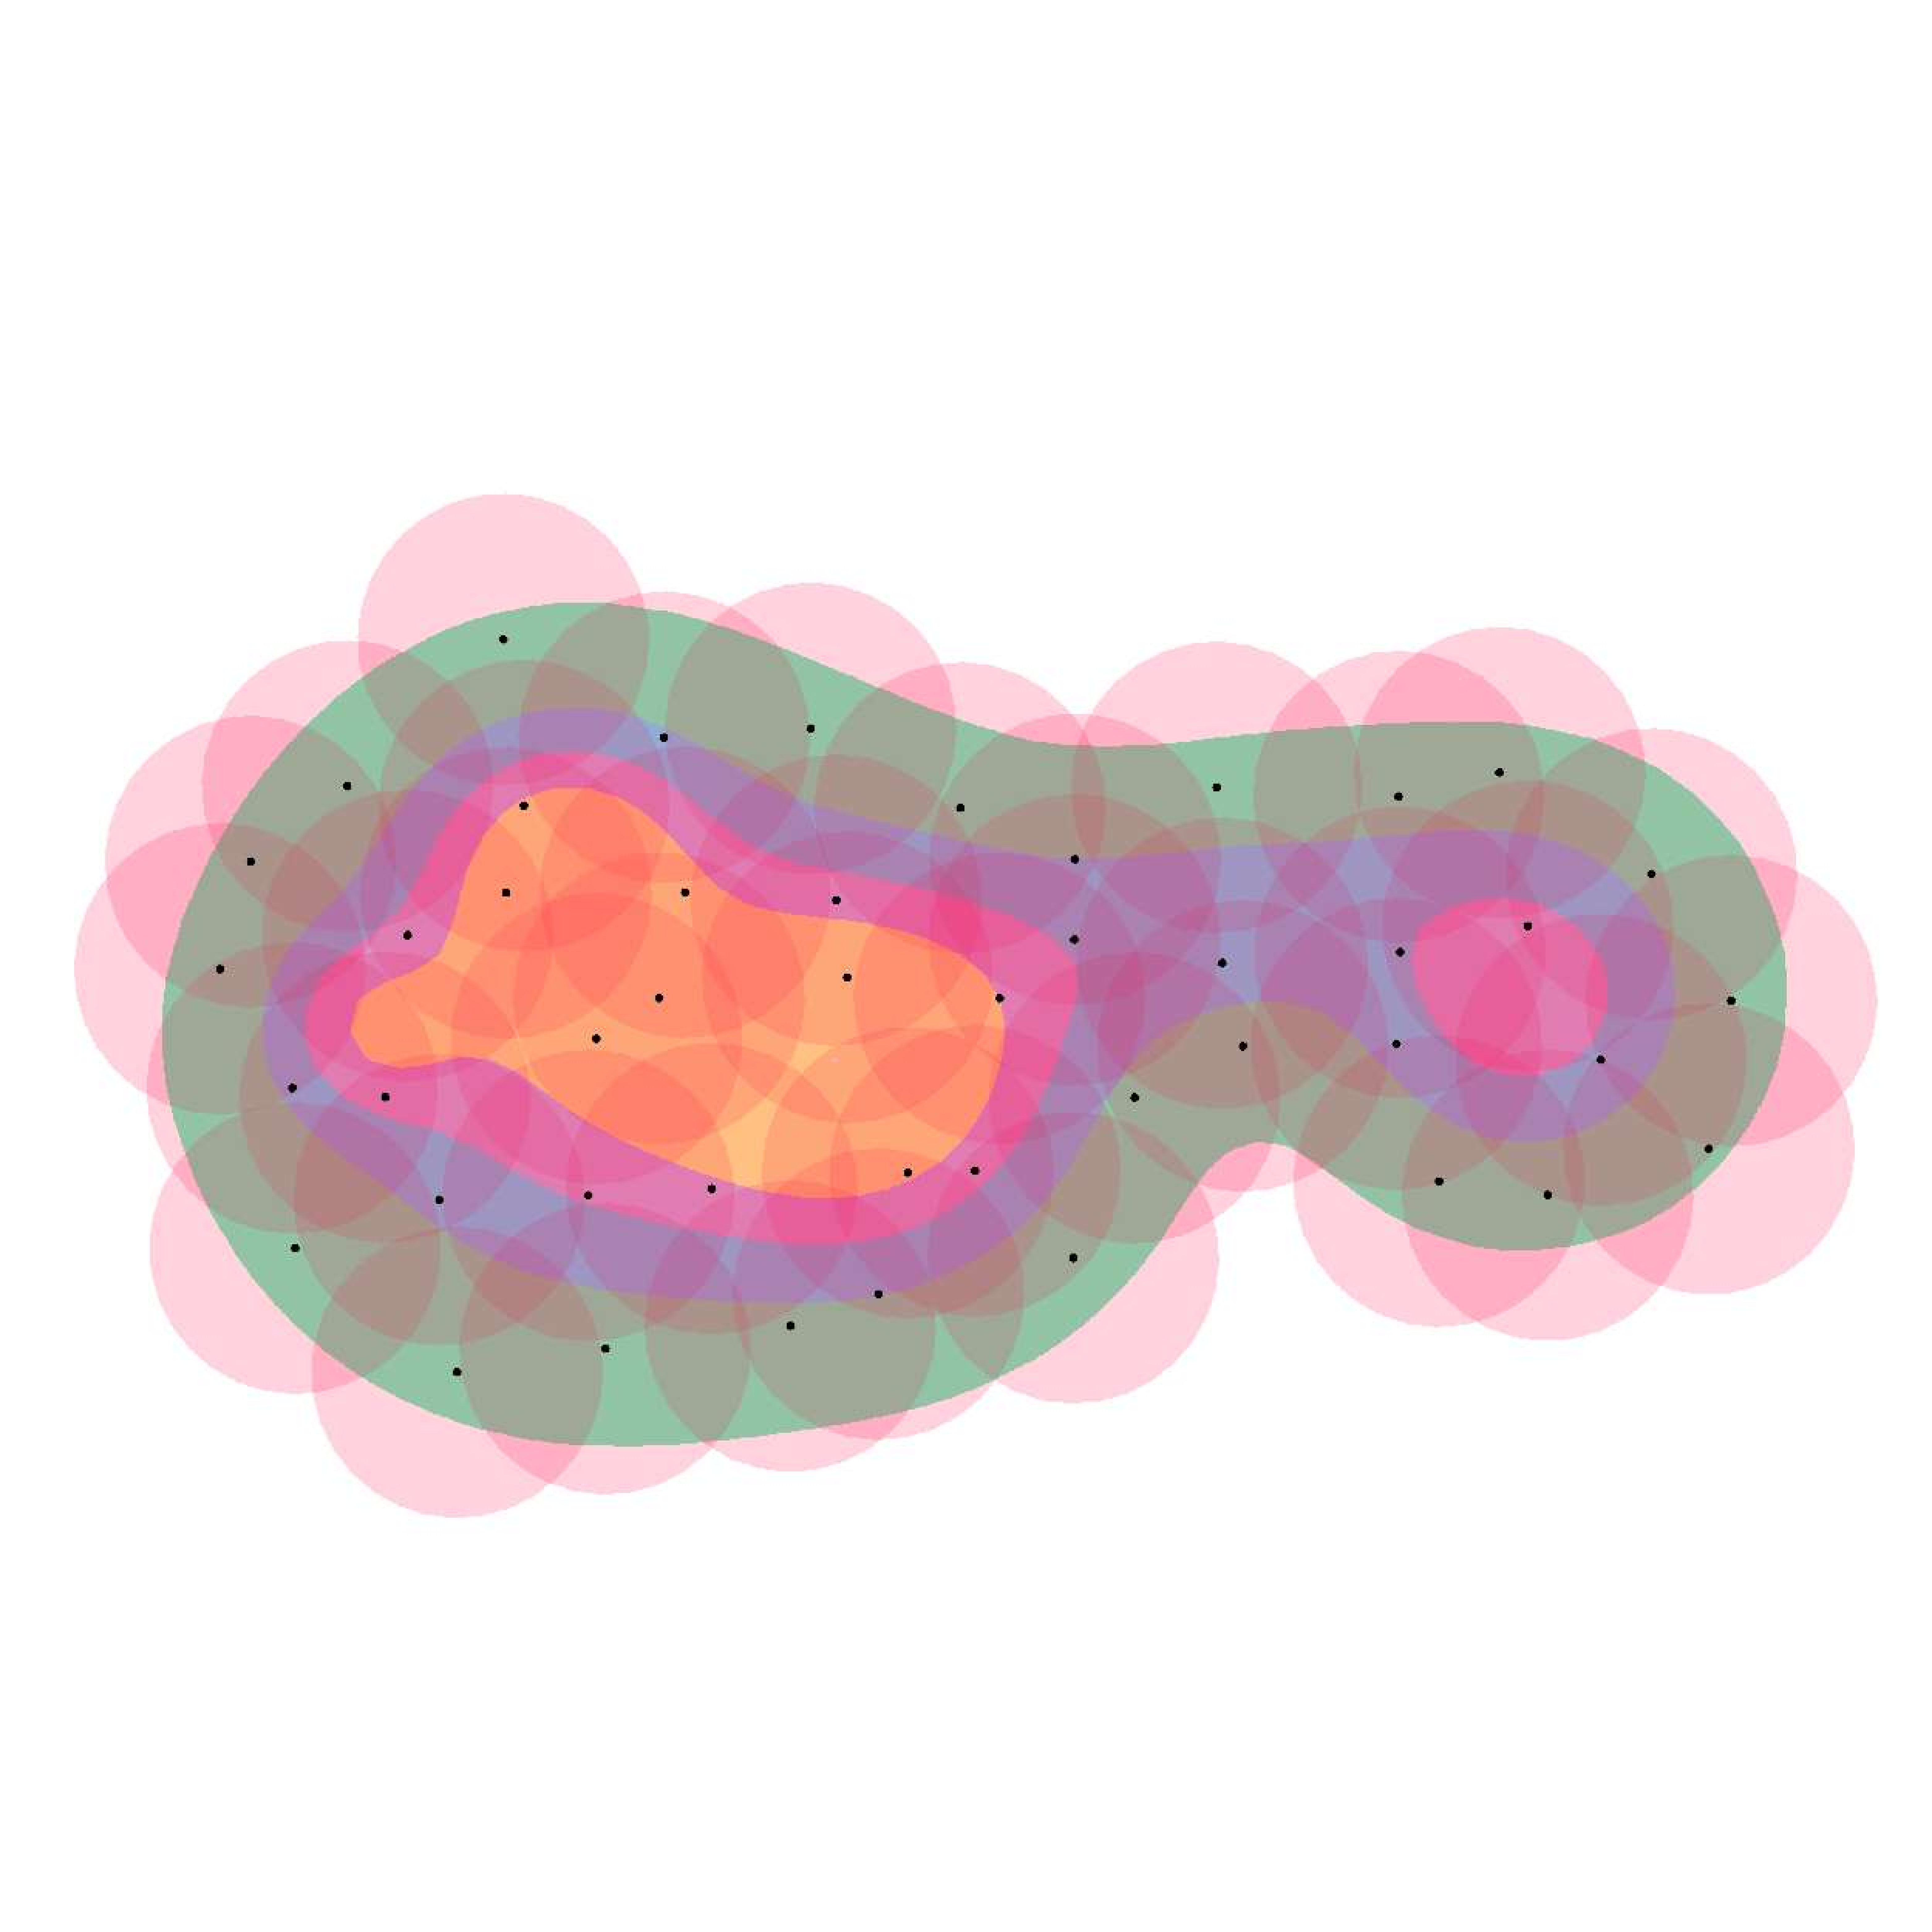
\includegraphics[trim=100 600 100 700, clip, width=0.4\linewidth]{figures/partial4/cover-comp.pdf}
  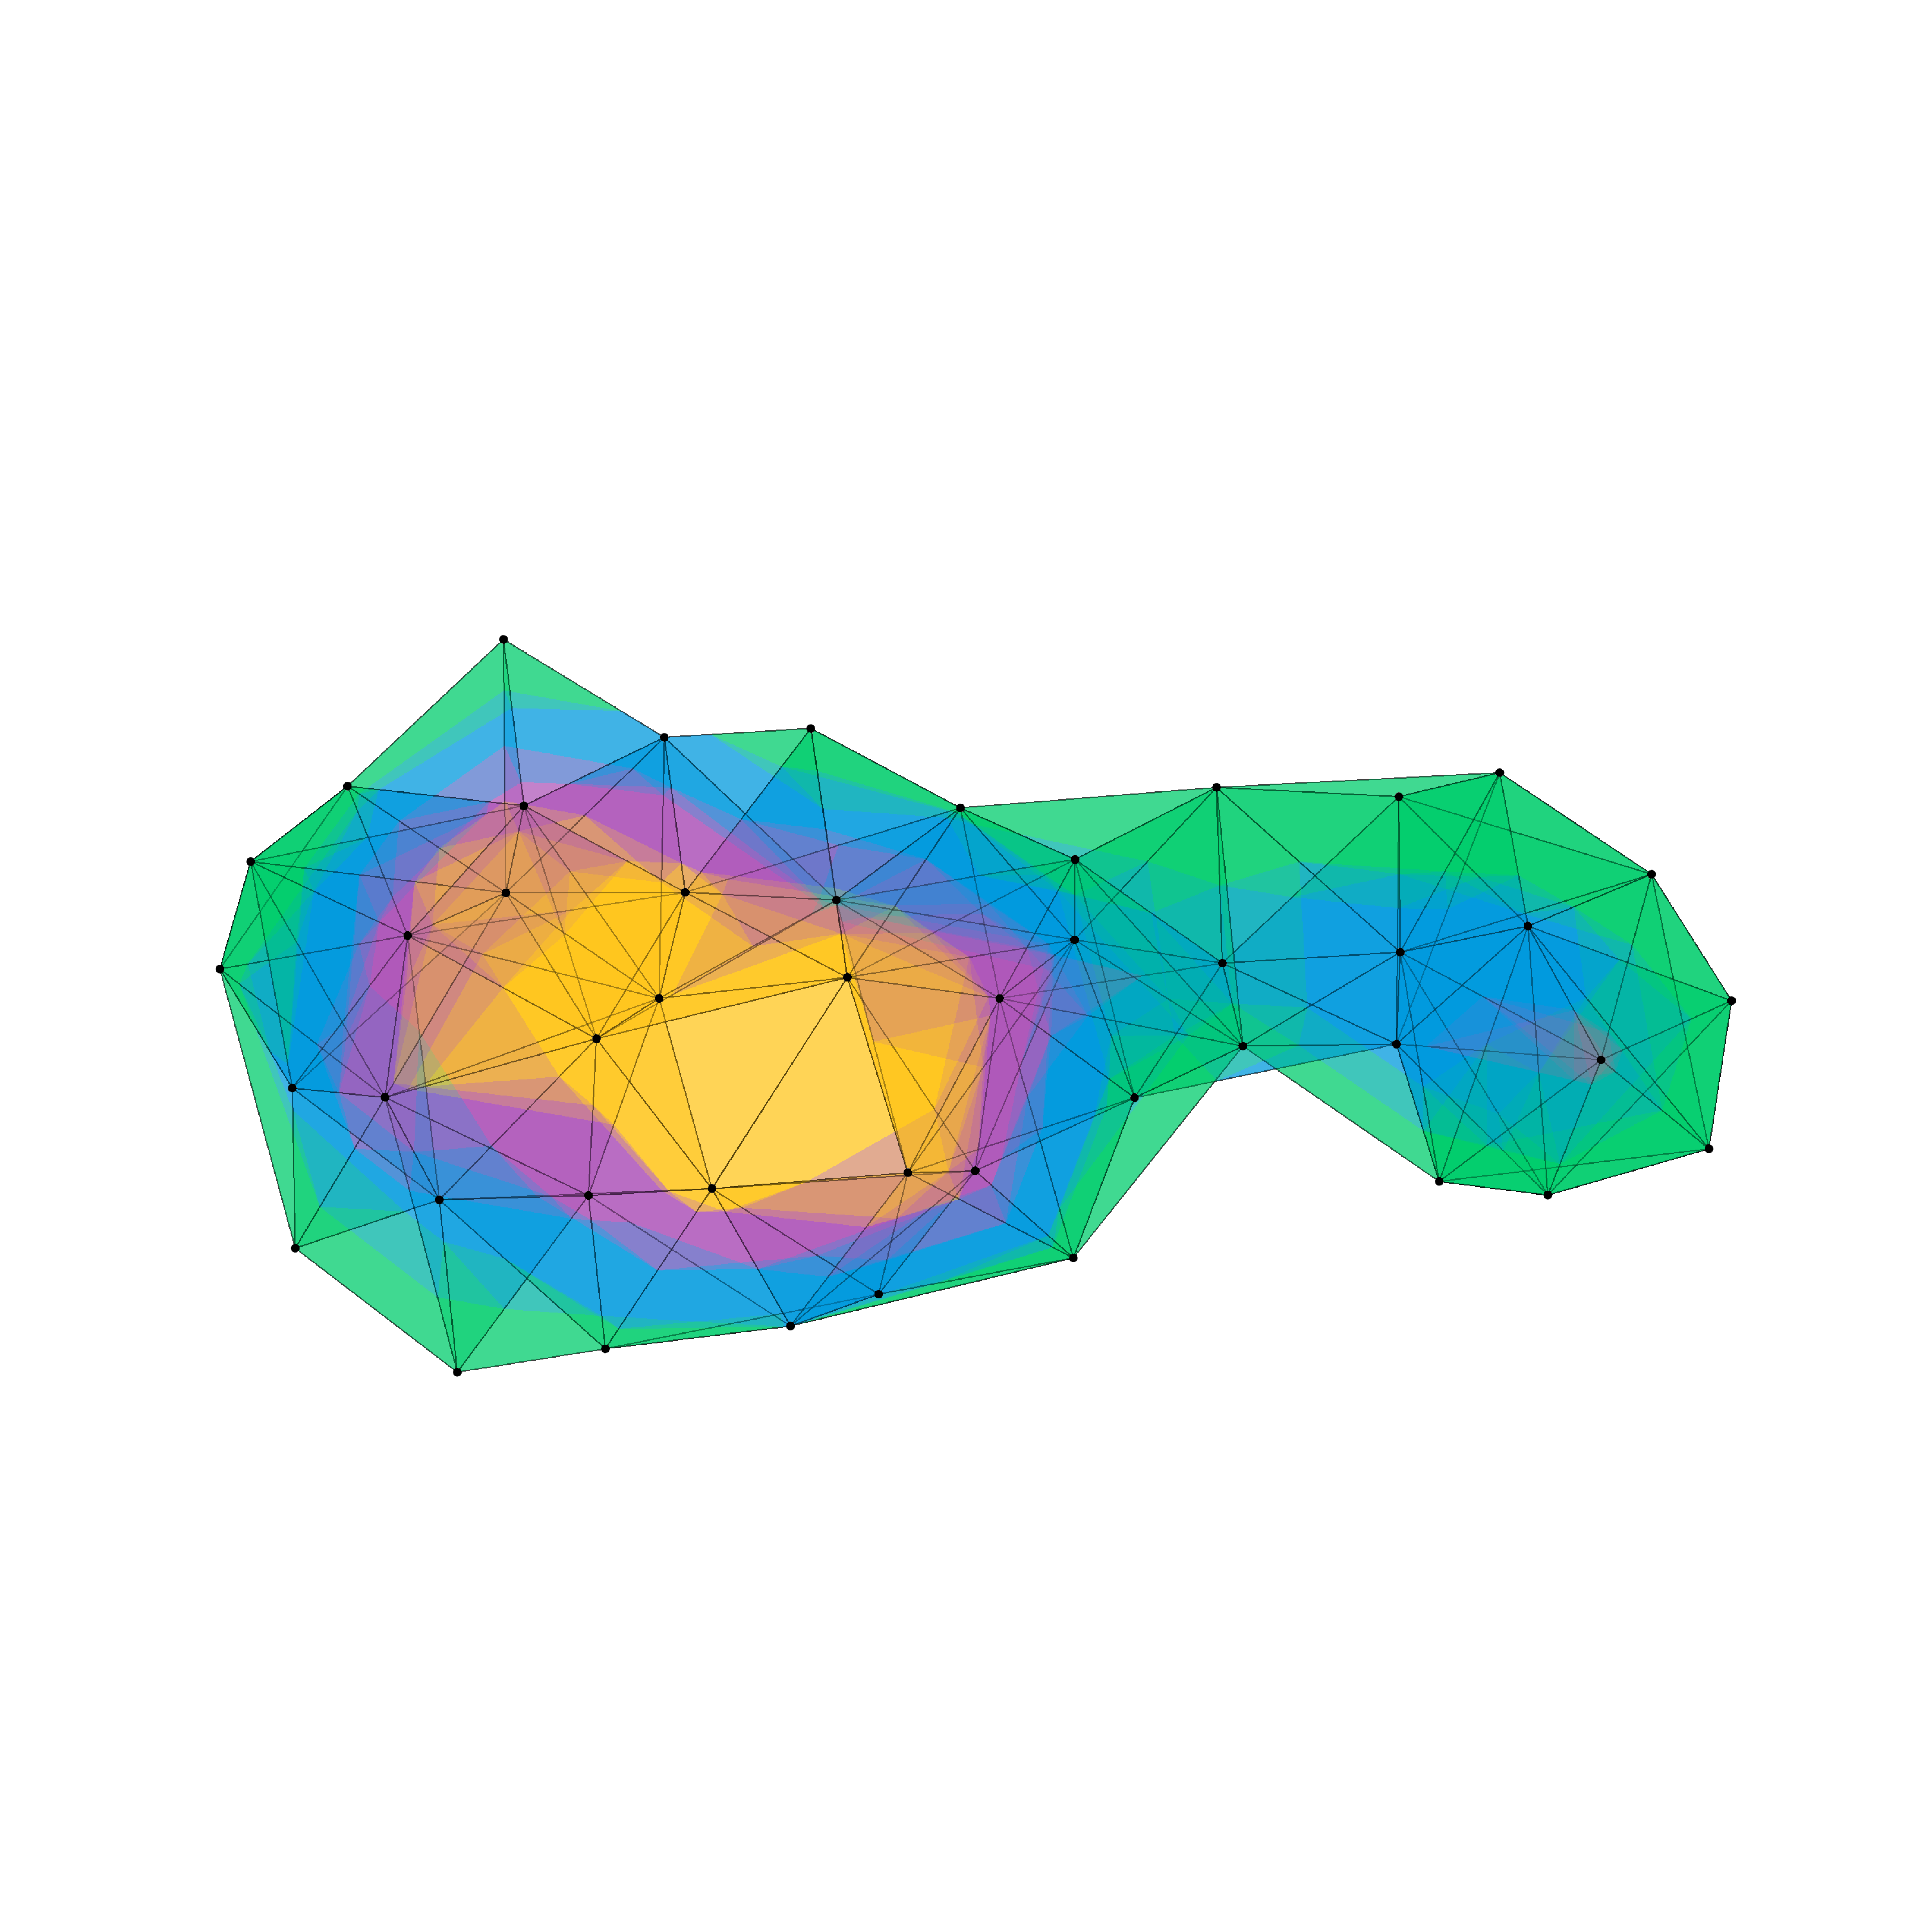
\includegraphics[trim=100 600 100 900, clip, width=0.4\linewidth]{figures/partial4/complex_nosurf.pdf}
  \caption{A cover of a scalar field and a simplicial complex used to approximate its persistent homology.}
\end{figure}
% \end{wrapfigure}
